\section{Results of simulations}\label{sec:results-of-simulations}
First, a baseline had to be found in which the system was stable.
That is finding settings where almost no meals were discarded, and no customers would leave.
Several automated runs were executed for one day ( 25 * 60 = 1440 tick).

The variables, with the default values, are:

\begin{center}
    \begin{tabular}{ |c|c| }
        \hline
        variable              & type \\
        \hline
        \hline
        number-of-restaurants & int  \\
        \hline
        number-of-customers   & int  \\
        \hline
        number-of-deliverers  & int  \\
        \hline
        prepair\_time\_mean   & int  \\
        \hline
        wait\_for\_deliverer  & int  \\
        \hline
    \end{tabular}
\end{center}

First, some runs with 25 and 50 deliverers were tried.
The results from figures ~\ref{fig:examples 25 deliverers} and ~\ref{fig:examples 50 deliverers} show that no differences between
25 and 50 deliverers.
The delivered meals are indicated with the orange line.
The reason for this is that the wait\_for\_deliverer is too short.
The deliverer has to drive towards the restaurant, and if it takes too long, the meal is discarded.

\begin{center}
    \begin{figure*}
        \centering
        \begin{subfigure}[m]{0.30\textwidth}
            \centering
            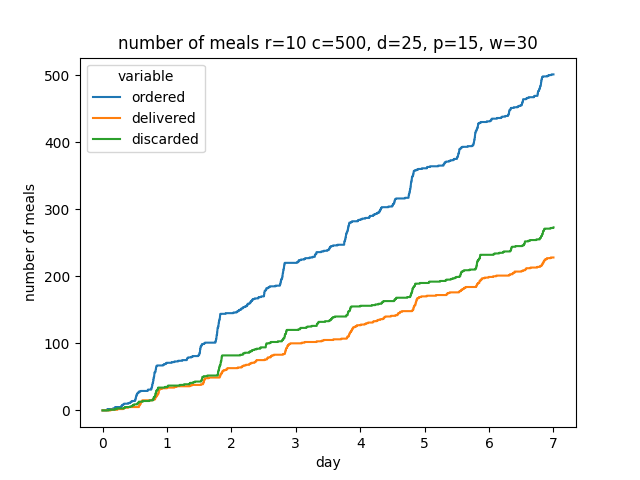
\includegraphics[width=\textwidth]{sections/run1/week_nd_1_food_ordering_distribution_500_10_25_30}
            \caption{example 1}
        \end{subfigure}
        \hfill
        \begin{subfigure}[m]{0.30\textwidth}
            \centering
            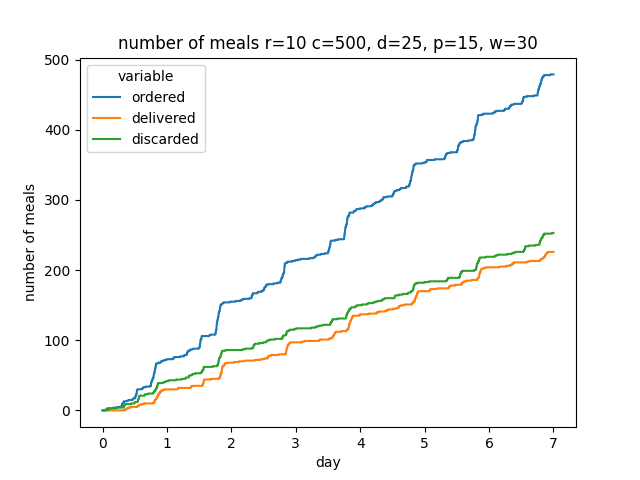
\includegraphics[width=\textwidth]{sections/run1/week_nd_2_food_ordering_distribution_500_10_25_30}
            \caption{example 2}
        \end{subfigure}
        \hfill
        \begin{subfigure}[m]{0.30\textwidth}
            \centering
            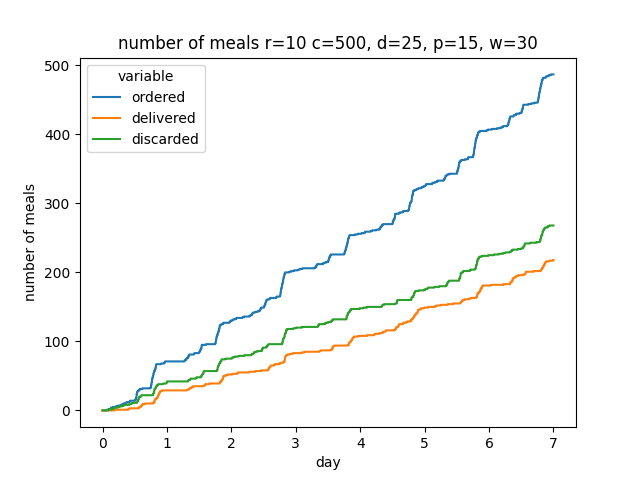
\includegraphics[width=\textwidth]{sections/run1/week_nd_3_food_ordering_distribution_500_10_25_30}
            \caption{example 3}
        \end{subfigure}
        \caption{Examples 25 deliverers}
        \label{fig:examples 25 deliverers}
    \end{figure*}
\end{center}
\begin{center}

    \begin{figure*}
        \centering
        \begin{subfigure}[m]{0.30\textwidth}
            \centering
            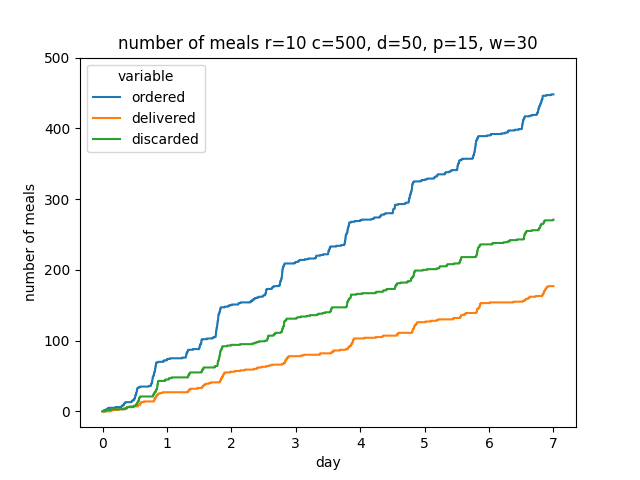
\includegraphics[width=\textwidth]{sections/run2/week_nd_1_food_ordering_distribution_500_10_50_30}
            \caption{example 1}
        \end{subfigure}
        \hfill
        \begin{subfigure}[m]{0.30\textwidth}
            \centering
            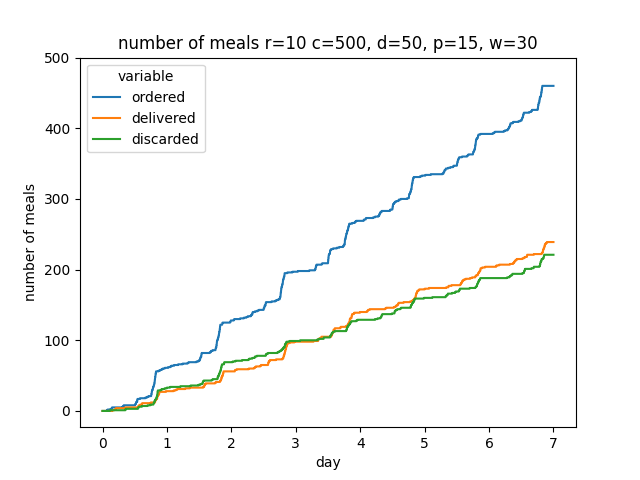
\includegraphics[width=\textwidth]{sections/run2/week_nd_2_food_ordering_distribution_500_10_50_30}
            \caption{example 2}
        \end{subfigure}
        \hfill
        \begin{subfigure}[m]{0.30\textwidth}
            \centering
            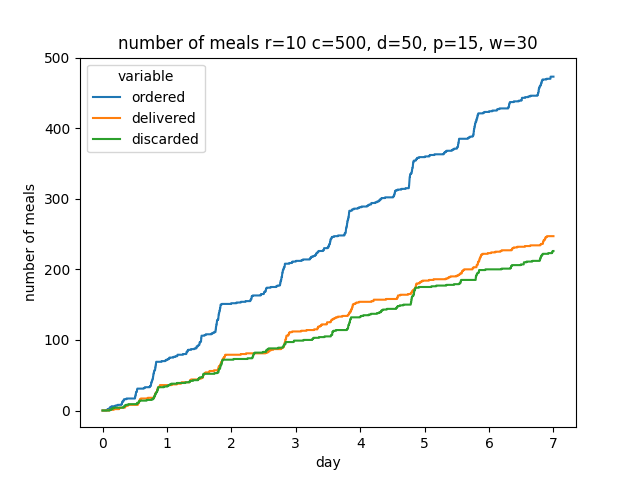
\includegraphics[width=\textwidth]{sections/run2/week_nd_3_food_ordering_distribution_500_10_50_30}
            \caption{example 3}
        \end{subfigure}
        \caption{Examples 50 deliverers}
        \label{fig:examples 50 deliverers}
    \end{figure*}
\end{center}

For the next run, the delivery times were longer.
The results are shown in figure~\ref{fig:examples 25 deliverers different wait time} and ~\ref{fig:examples 50 deliverers different wait time}
There is a difference: the longer the allowed wait time, the more meals are delivered and not discarded.

\begin{center}
    \begin{figure*}
        \centering
        \begin{subfigure}[m]{0.30\textwidth}
            \centering
            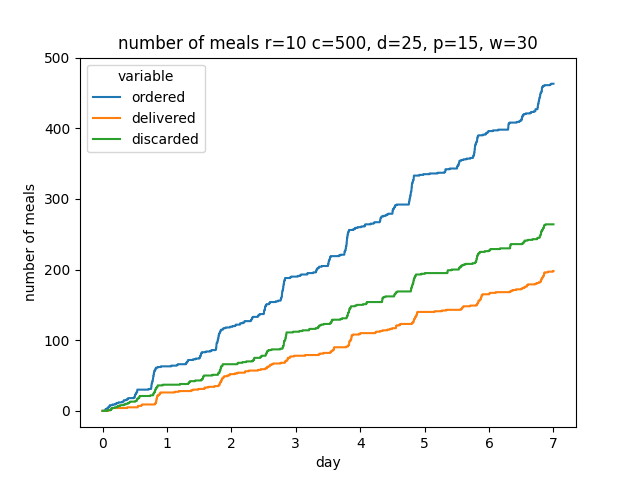
\includegraphics[width=\textwidth]{sections/run3/week_nd_1_food_ordering_distribution_500_10_25_30}
            \caption{30 min wait time}
        \end{subfigure}
        \hfill
        \begin{subfigure}[m]{0.30\textwidth}
            \centering
            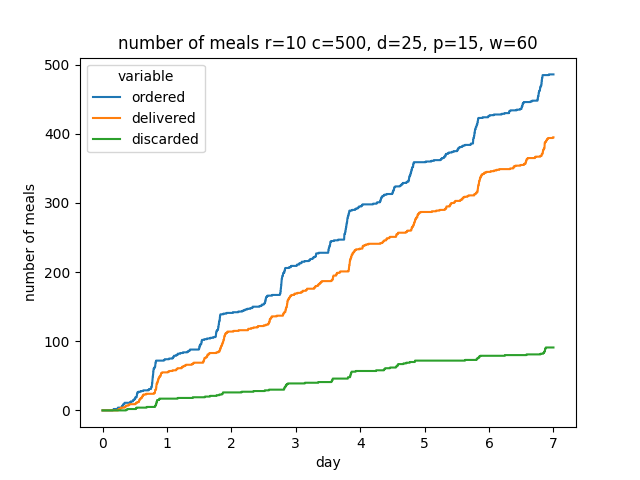
\includegraphics[width=\textwidth]{sections/run3/week_nd_2_food_ordering_distribution_500_10_25_60}
            \caption{60 min wait time}
        \end{subfigure}
        \hfill
        \begin{subfigure}[m]{0.30\textwidth}
            \centering
            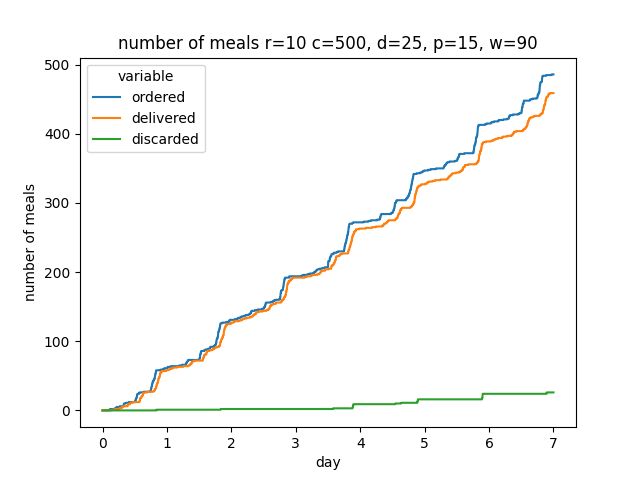
\includegraphics[width=\textwidth]{sections/run3/week_nd_3_food_ordering_distribution_500_10_25_90}
            \caption{90 min wait time}
        \end{subfigure}
        \caption{Examples 25 deliverers}
        \label{fig:examples 25 deliverers different wait time}
    \end{figure*}
\end{center}
\begin{center}

    \begin{figure*}
        \centering
        \begin{subfigure}[m]{0.30\textwidth}
            \centering
            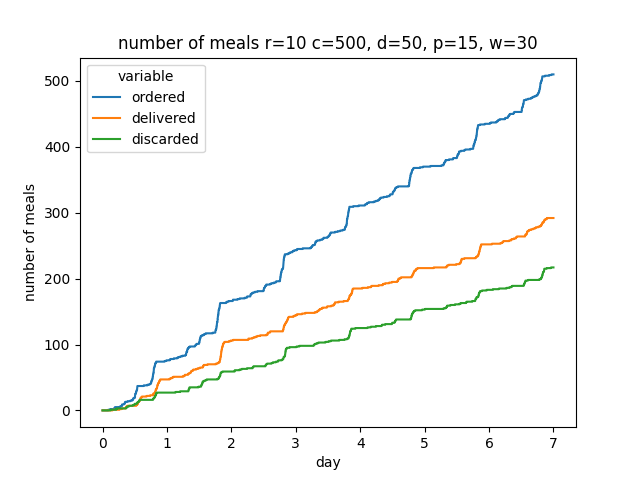
\includegraphics[width=\textwidth]{sections/run4/week_nd_1_food_ordering_distribution_500_10_50_30}
            \caption{30 min wait time}
        \end{subfigure}
        \hfill
        \begin{subfigure}[m]{0.30\textwidth}
            \centering
            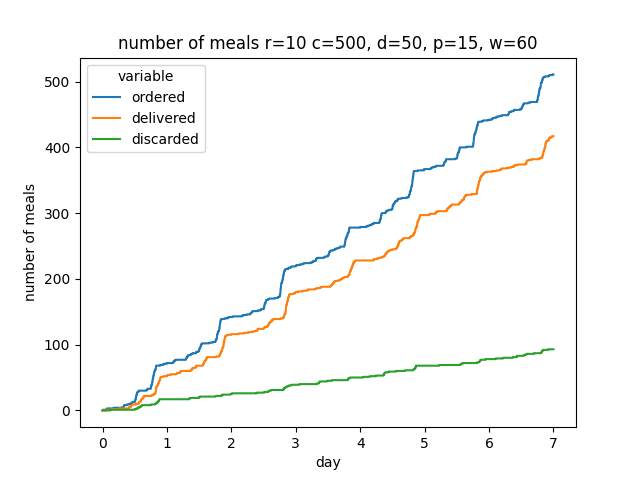
\includegraphics[width=\textwidth]{sections/run4/week_nd_2_food_ordering_distribution_500_10_50_60}
            \caption{60 min wait time}
        \end{subfigure}
        \hfill
        \begin{subfigure}[m]{0.30\textwidth}
            \centering
            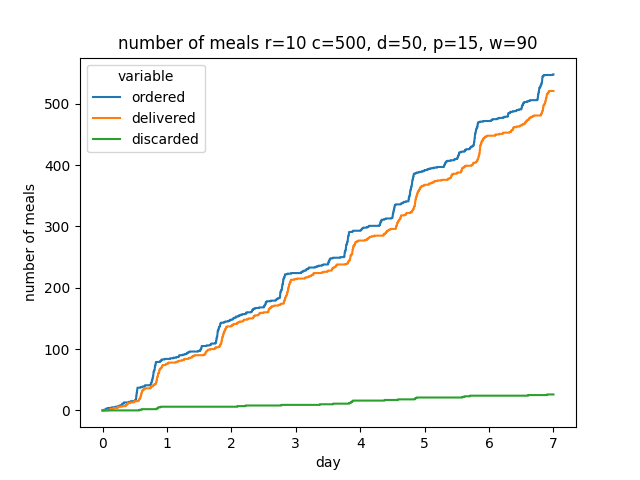
\includegraphics[width=\textwidth]{sections/run4/week_nd_3_food_ordering_distribution_500_10_50_90}
            \caption{90 min wait time}
        \end{subfigure}
        \caption{Examples 50 deliverers}
        \label{fig:examples 50 deliverers different wait time}
    \end{figure*}
\end{center}

We can tell from these results that the longer the waiting time, the more deliveries are made,
Again, there is not much difference between the number of deliverers.

To find out what the effect is of the number of deliverers, the simulation was run for a waiting time of 60 and 90 minutes,
and 10 to 60 deliverers.
The result of these simulations, for a simulated week, are:

\begin{center}
    \begin{tabular}{ |c|c|c| }
        \hline
        waittime       & 60   & 90   \\
        nr. deliverers &      &      \\
        \hline
        \hline
        10             & 63\% & 69\% \\
        \hline
        20             & 75\% & 88\% \\
        \hline
        30             & 83\% & 96\% \\
        \hline
        40             & 87\% & 99\% \\
        \hline
        50             & 89\% & 97\% \\
        \hline
        60             & 80\% & 99\% \\
        \hline
    \end{tabular}
\end{center}

With this information, the baseline is set.
The best result would be a wait time of 90 minutes and 30 deliverers; more deliverers would have the same result.

\subsection{Model variant 1}\label{subsec:model-variant-1}
The baseline is determined with the next settings:
\begin{center}
    \begin{tabular}{ |c|c|c| }
        \hline
        variable              & type & default \\
        \hline
        \hline
        number-of-restaurants & int  & 10      \\
        \hline
        number-of-customers   & int  & 500     \\
        \hline
        number-of-deliverers  & int  & 30      \\
        \hline
        prepair\_time\_mean   & int  & 15      \\
        \hline
        wait\_for\_deliverer  & int  & 90      \\
        \hline
    \end{tabular}
\end{center}

Now, simulations will be run over a much longer period, and the number of meals delivered per deliverer will also be measured.

On six runs of simulated ten weeks, the results are:

\begin{center}
    \begin{tabular}{ |c|c|c|c| }
        \hline
        meals & meals & meals & percentage \\
        ordered & delivered & discarded & delivered \\
        \hline
        \hline
        4857          & 4798           & 58             & 0.98                 \\
        \hline
        4839          & 4755           & 81             & 0.98                 \\
        \hline
        4958          & 4630           & 327             & 0.93                 \\
        \hline
        4773          & 4645           & 126             & 0.97                 \\
        \hline
        4895          & 4562           & 330             & 0.93                 \\
        \hline
        4800          & 4756           & 41             & 0.99                 \\
        \hline
        \hline
        4853          & 4691           & 160             & 0.96 \\
        \hline
    \end{tabular}
\end{center}

A deliverer delivers an average of 4691 meals per day, or (10 * 7 * 24 + 60 * 30) = 2.23 meals.

\subsection{Model variant 2}\label{subsec:model-variant-2}
For the second variant, deliverers may leave if they don't make enough money; in this setting, only the number of deliveries is counted for simplicity.

In the previous section, a deliverer may have heard that a deliverer can deliver 2.34 meals per day or 15.63 per week.

In this model, if a deliverer delivers less than this number, rounded to 15, in a week, they will stop delivering.
The delivery company knows it can deliver 4691 in 10 weeks and expects this from this system.

The simulation is rerun for ten weeks.

The following table contains the results:
\begin{center}
    \begin{tabular}{ |c|c|c|c|c| }
        \hline
        meals & meals & meals & percentage & remaining \\
        ordered & delivered & discarded & delivered & deliverers \\
        \hline
        \hline
        4724          & 4231           & 491             & 0.89  & 18               \\
        \hline
        4861          & 4231           & 573             & 0.88  & 19               \\
        \hline
        4913          & 4386           & 524             & 0.89  & 19               \\
        \hline
        4773          & 3880           & 832             & 0.82  & 14               \\
        \hline
        4712          & 4508           & 406             & 0.91  & 22               \\
        \hline
        4917          & 4266           & 595             & 0.87  & 19               \\
        \hline
        \hline
        4831          & 4250           & 570             & 0.88  & 19               \\
        \hline
    \end{tabular}
\end{center}

The average number of meals delivered in 10 weeks is much lower, but the number of remaining deliverers is also much lower.

What is interesting is to see what the average number of meals delivered per deliverer is over the weeks; this is shown in figure~\ref{fig:average}.

\begin{figure*}
\centering
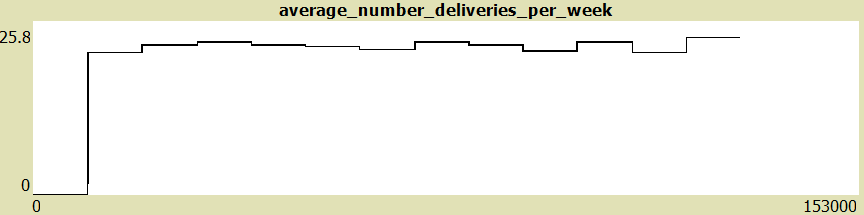
\includegraphics[width=12cm]{sections/pics/average}
\caption{NetLogo  graph containing average deliveries per deliverer per week.}
\label{fig:average}
\end{figure*}

This graph shows that because many deliverers drop out in the beginning, the average for the remaining deliverers is higher compared to Model 1.

The result of this simulation is that giving deliverers a steady job will increase the number of meals delivered for the company.
However, the average per deliverer is lower than in a system where deliverers can decide to leave if the deliveries are less than those for a certain job.

Because more deliveries occur, the company could even pay them less per delivery and keep them onboard.

Of course, this is a highly abstract world, but it does say something about why delivery companies prefer the latter system.
It is also, on average, more profitable for the deliverers who remain, but not for the ones who left, of course.

\subsection{Conclusion}\label{subsec:conclusion}
A model has been created in NetLogo. It works as intended and reflects the delivery process in a very abstracted way.
Other researchers may use and adapt the model freely.

The simulations indicate that seeing the deliverers as independent contractors who stay when they earn enough is more advantageous to the companies and the deliverers.
But this says nothing about other factors like safety, sick leave, and working conditions.
More deliveries also mean more manual work; deliverers may get fatigued and risk their safety.

Luckily, in the real world, a combination exists: working for a lower solid income and getting a bonus for each delivery.






